%%%% PRE-AMBLE (load packages, set preferences, etc.)
\documentclass{article}
\usepackage[utf8]{inputenc}
\usepackage{amsfonts,amssymb,amsthm,amsmath,graphicx,array,biblatex,enumitem}
\usepackage[skip=2pt,font=scriptsize]{caption}
\usepackage[lmargin=1in,rmargin=1in,tmargin=1in,bmargin=1in]{geometry}
\newtheorem{theorem}{Theorem}[section]
\graphicspath{ {images/} }
\addbibresource{thesis_references.bib}


%% DEVELOP TITLE CONTENT
\title{Furthering Usability and Efficiency of Massively Parallel Gaussian Process Regression as Applied to Multi-Beam Sonar Data}
\author{
    by\\~\\
    Phillip M. Parisi\\
    Department of Ocean Engineering\\
    University of Rhode Island\\
    philparisi@uri.edu}
    
\date{October 2022}

%%%% BEGIN DOCUMENT
\begin{document} % set 'environment' to 'document'

%%%% TITLE PAGE
\maketitle %inserts title defined in preamble
\thispagestyle{empty}

% thesis proposal required text
\begin{center}
\bigskip \bigskip \bigskip \bigskip \bigskip \bigskip \bigskip \bigskip
A THESIS PROPOSAL SUBMITTED IN PARTIAL FULFILLMENT OF THE REQUIREMENT FOR THE DEGREE OF \\~\\ MASTER OF SCIENCE \\~\\ IN \\~\\ OCEAN ENGINEERING
\end{center}
\pagebreak

%%%% FIGURES & TABLES
%\thispagestyle{empty}
%\listoffigures
%\listoftables
%\newpage
%\pagenumbering{arabic}

%%%% STATEMENT OF PROBLEM
\pagenumbering{arabic} % start page numbering

\section{Statement of Problem}
Gaussian Process Regression (GPR) is a supervised machine learning approach for learning input-output mappings from training data (Rasmussen, 2006). GPRs can generate estimates at new prediction points along with the associated uncertainties.  The underlying computation, however, suffers from mathematical inefficiencies (e.g. the inverse operation requiring $O({N^3})$ time complexity) which renders the most basic implementation of a GPR intractable for large data volumes (Rasmussen, 2006). Krasnosky (2021) introduced a parallel computational framework to speed up the algorithm, leading to an online GPR solution that generates a terrain model with uncertainties from a set of input points collected in a push broom manner. GPR was shown to improve the resolution of seafloor terrain models made from multibeam sonar data and can generate an uncertainty model which other standard mapping methods (splines, gridded, polynomial, etc.) lack (Krasnosky, 2021).

\begin{figure}[htp]
    \centering
    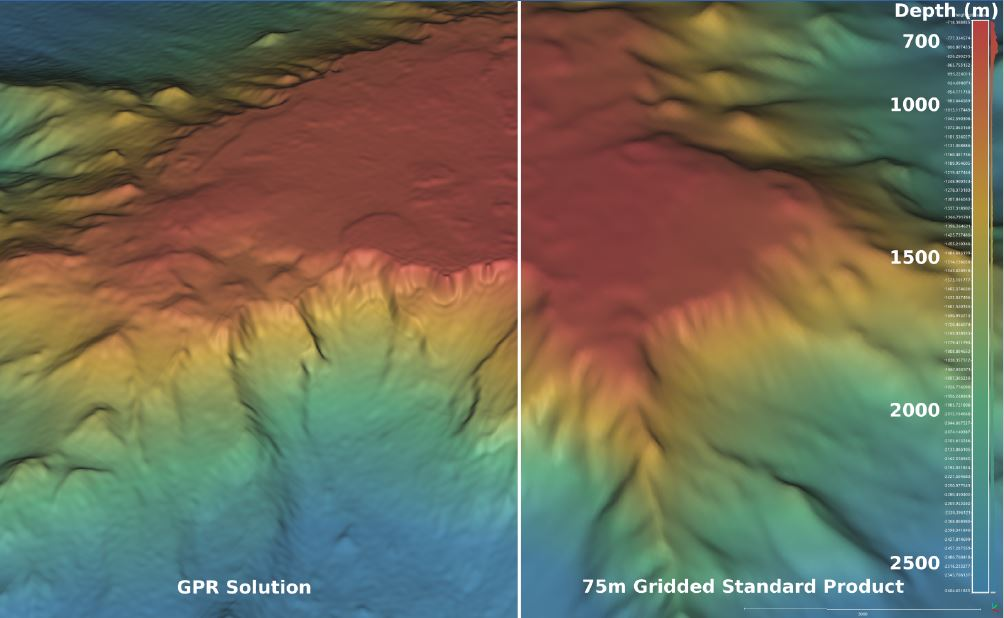
\includegraphics[width=16cm]{Krasno_GPRvsStandard.jpg} %filename and border
    \caption[GPR is great]{Bathymetry maps produced using MP-GPR (left) and the standard 75mm gridding method (right). Higher resolution is evident in the GPR. Figure from Krasnosky (2021).} 
    \label{fig:kk} %unsure what this is used for
\end{figure}

Krasnosky's (2021) Massively Parallel Gaussian Process Regression (MP-GPR) offers numerous computational speed-ups, namely an approximation to the kernel function, usage of a graphics processing unit (GPU) to perform mathematical operations, and iterative matrix updates that incorporate new bathymetric data as an input stream. While MP-GPR made standard GPR tractable on sonar data it still requires computationally robust hardware (high-end GPUs) and suffers from inefficient kernel hyperparameter optimization (Krasnosky, 2021). The hyperparameters within the GPR define the anticipated length scale and variance of the input points and can be optimized based on the data. Additionally, bathymetric data can be over-sampled during certain collection scenarios (e.g. ship turns will result in high point density) where an intelligent reduction of training data could substantially decrease computation time with a minor reduction in model accuracy. 
%\pagebreak


%%%% JUSTIFICATION FOR AND SIGNIFICANCE OF STUDY

\section{Justification for and Significance of Study}
GPR has been applied to underwater terrain modeling (Barkby, 2012), terrain aided navigation (TAN) (Hitchcox and Forbes, 2020), and simultaneous localization and mapping (SLAM) (Ma et al., 2018). Utilizing a GPU to compute GPR solutions has also been explored (Franey et al., 2012; Gramacy et al., 2014).  However, these methods sought GPR solutions as a post-processing tool. Krasnosky's (2021) MP-GPR proposed an online updateable GPR model that leveraged parallel processor cores on a GPU for real-time bathymetric map generation. This MP-GPR terrain model was paired with a bathymetric distributed particle SLAM (BPSLAM) (Barkby et al., 2012) method to produce the novel GPU-based extension of BPSLAM (GP-BPSLAM) (Krasnosky, 2021).

MP-GPR and GP-BPSLAM run in real-time but require significant computer power (e.g. a NVIDIA 2080ti GPU with 4352 CUDA cores). Modern mobile platforms, such as autonomous underwater/surface vehicles (AUVs/ASVs), are unlikely to possess high-end GPUs due to their significant power consumption.  With ever increasing sensor resolution and acquisition rates, there is a need to further reduce GPR compute time for real-time performance on a wide-range of hardware, such as the smaller NVIDIA Jetson NX Xavier, to make MP-GPR broadly applicable and relatively platform agnostic (Krasnosky, 2021).

GPR has also been employed to map environmental variables, such as radiation (West et al., 2021). The development of spatial and temporal maps of environmental variables (e.g. temperature, salinity) would benefit from an efficient GPR solution. Field data gathered by mobile devices or sensors moving in 3D space is susceptible to transient changes in environmental conditions, yet modern mapping methods are unable to appropriately express the time domain. A robust approximate MP-GPR framework including time would enable development of online spatiotemporal maps. Notably, projects similar to the Rhode Island Consortium for Coastal Ecology Assessment Innovation and Modeling (RI C-AIM) would find value in such maps created for Narragansett Bay.

%\pagebreak


%%%% METHODOLOGY AND PROCEDURES
\section{Methodology and Procedures}

\subsection{Gaussian Process Regression}
Empirical data points $D$ from a set of $N$ observations, known as \textit{training data}, consists of inputs $\boldsymbol{x}$ and corresponding targets $\boldsymbol{y}$. Each observation $\boldsymbol{x}_i$ of $d$ dimensions maps to a scalar target $y_i$, which is a noisy realization of the underlying function $f$. 
That is,

\begin{gather*}
    D = \{(\boldsymbol{x}_i,y_i)|i=1,\ldots,N\} \\
    \boldsymbol{x}\in\mathbb{R}^{N \times d}, \boldsymbol{y} \in\mathbb{R}^{N}, y_i = f(\boldsymbol{x}_i) + \epsilon,
\end{gather*}

where $\epsilon$ denotes error. When applied to seafloor mapping, $\boldsymbol{x}_i = (\mathrm{northing}, \mathrm{easting})$ and $y_i = \mathrm{depth}$. During the training portion of the problem, $D$ is used to learn the underlying function $f$.  During the inference step, $f$ is used to predict depth $\boldsymbol{y}^*$ over a new set of geographically dense inputs $\boldsymbol{x^*}$ to form a map.

An important component of any GPR model is the kernel. A commonly used kernel is the squared exponential (SE) kernel:
\begin{equation}
    k(\boldsymbol{x},\boldsymbol{x'}) = \sigma_f^2 exp(-\frac{|\boldsymbol{x}-\boldsymbol{x'}|^2}{2l^2}),
\end{equation}
where $|\boldsymbol{x}-\boldsymbol{x'}|$ denotes the magnitude of the difference between vectors $\boldsymbol{x}$ and $\boldsymbol{x'}$, and $\boldsymbol{\theta} = \{l,\sigma_f^2\}$ are hyper-parameters. MP-GPR utilizes an approximation to the SE kernel which incorporates the same hyper-parameters.

\subsection{Approximate Methods}
In general, a multitude of ``approximate methods" have been developed to reduce GPR compute time for regression and classification.  As standard GPR scales with $O({N^3})$, most approximate methods fabricate a representative data set $D_R$ containing $M$ points, where $M \ll N$. $D_R$ can be composed of a subset from the training data $D$ or of newly generated pseudo-data points that may not be present in $D$, such that $D_R \not\subset D$. $D_R$ then serves as the training data for the model in lieu of $D$, decreasing algorithm time complexity and reducing model accuracy to various degrees. Selecting points from $D$ to form $D_R$ will be referred to as \textit{downsampling}.

The Subset of Data (SD) family of approximate methods select a sample of the training data to pass to the model which uses the standard GPR inference equations. Notable SD candidates include uniform random downsampling, systematic downsampling, and heuristic-based methods such as entropy change $\Delta h$ (Lawrence and Platt, 2004) and information gain $\Delta i$ (Seeger et. al., 2003). SD time complexity is $O({M^3})$.  Projected Processes (PP) include an extension of entropy change and information gain that incorporate information from all $N$ training points into the GPR inference equations. PP methods have a time complexity of $O({NM^2})$. Lastly, joint optimization methods, which select pseudo-points for $D_R$ and hyperparameters concurrently, are effective yet require an alternative problem formulation to GPR and will not be considered in this study. All methods face the cost of choosing the points in $D_R$; hence, cheap (``greedy'') selection criteria are desired (Rasmussen, 2006). Additionally, every method requires a retuning of hyperparameters to account for the modified training data.

\subsection{Approaches in this Study}
The goal of this study is to determine the ``best" approximate method for online seafloor mapping. Extensions will be built onto Krasnosky's GPR code base, and testing will be performed using data from surveys previously completed by the Roman Marine Robotics Lab. 

SD approximate methods will be explored first, followed by PP if needed. MP-GPR arranges live survey data spatially into ``blocks" which are passed to the on-board GPU for processing. The approximate methods will be implemented at the block level of the algorithm as ``blockulators'' that select which points from incoming sonar pings will be included into the next block ($D \rightarrow D_R$). There is an inherent trade off between algorithm accuracy and speed when selecting the percentage of points that remain in $D_R$. This \textit{downsample percent} parameter will require tuning for each approximate method and subsequent retraining of hyperparameters. The study will seek to find the approximate method that offers the greatest runtime reduction while maintaining an acceptable level of accuracy relative to the full solution. 

The following approximate methods are examples of what may be implemented (non-exhaustive list):

\begin{itemize}[noitemsep]
    \item a \textit{Uniform Random} SD method that exploits a uniform random distribution to select points,
    \item a \textit{Systematic} SD method that selects every $j$th point,
    \item a \textit{Random Hybrid} SD method that combines systematic and uniform random selection,
    \item an \textit{Information Gain} SD or PP method that uses a heuristic to informatively select points.
\end{itemize}

\begin{figure}[htp]
    \centering
    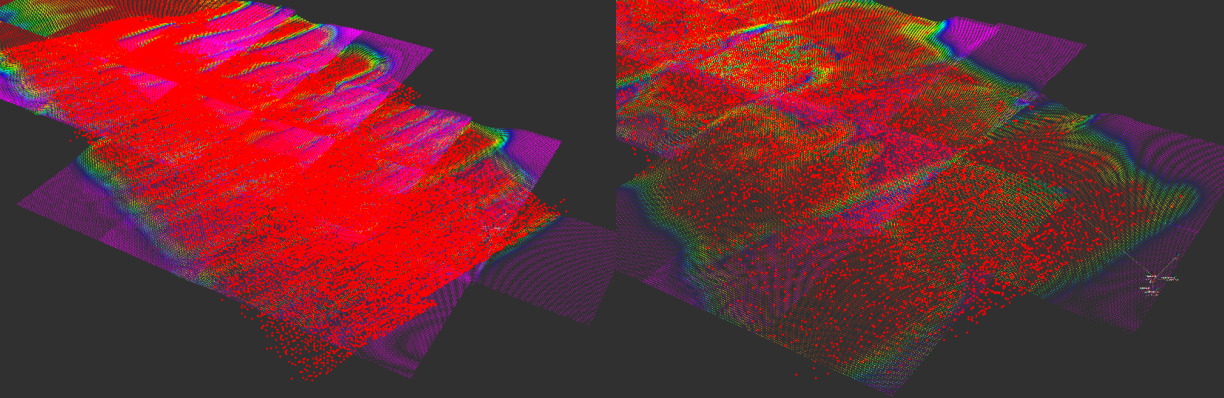
\includegraphics[width=15
    cm]{GPR_comparison_Fullto10.png} %filename and border
    \caption[Standard vs. Downsample]{Initial results comparing a Standard GPR solution (left) to the Random Downsampling Approximate Method (right) with \textit{downsample percent} set to 0.1. Each red point represents a sonar sounding. Colored blocks visualize the GPR solution calculated over a given block of points.} 
    \label{fig: a10} %unsure what this is used for
\end{figure}

Each candidate method will first be tested in MATLAB and trained on two-dimensional data ($\boldsymbol{x},\boldsymbol{y}\in\mathbb{R}^{N}$). Then, the method will be implemented in C++ as a blockulator in the existing MP-GPR code base. Numerous speed tests will be run to calculate the average runtime of the approximate method. Each run will generate the same set of prediction points, which will be compared against the predictions of standard GPR as a baseline. Two metrics will be computed: computational speed-up, $T_x$, and coefficient of determination $R^2$. The $M$ points included in $D_R$ (such that $M/N = \textit{downsample percent}$) can be varied to find the maximum $T_x$ that can keep $R^2$ above a threshold (e.g. $R^2 \geq 0.95$). It is expected that as $M$ decreases, $T_x$ will increase while $R^2$ decreases. Initial experimentation has shown curves similar to Figure 1, though alternative behavior may be seen upon implementation. Error statistics, such as mean absolute error (MAE) or mean squared error (MSE), may be used to quantify error alongside the coefficient of determination. 

\begin{figure}[htp]
    \centering
    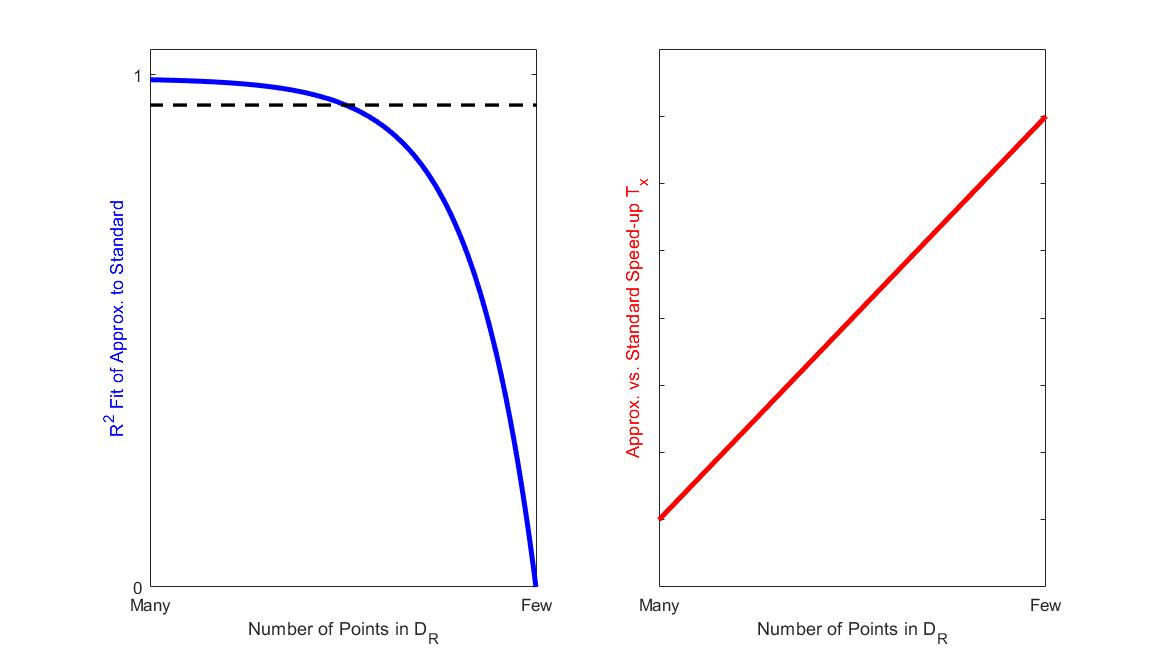
\includegraphics[width=12cm]{TheoreticalSpeedup_R2_forThesisProposal_general.jpg} %filename and border
    \caption[Expected Speed-up]{Experimental behavior as the points in $D_R$ decrease for the systematic selection method. It is expected that the $R^2$ fit (left) exhibits a decrease with an exponential term. Methods must stay above an acceptable threshold (shown at 0.95). $T_x$ (right) is expected to increase as fewer data points are included in $D_R$.}
    \label{fig: mc} %unsure what this is used for
\end{figure}

After running trials on each method, a side-by-side comparison of the various methods will be feasible.  Determination of the fastest GPR approximate method that stays above the accuracy threshold will conclude this study.  Online field testing may ensue, time and weather permitting. 

%\pagebreak


%%%% RESOURCES REQUIRED
\section{Resources Required}

The resources required for the project are:
\begin{enumerate}
    \item MP-GPR code. Code base access has been granted via Bitbucket and initial simulations were executed. All package dependencies are open source and accessible. 
    \item Laptop and/or desktop with a graphics processing unit (GPU). The Roman Marine Robotics Lab currently has these machines available.
    \item Bathymetric survey data in .rosbag format.  Data is accessible and has been obtained.
    \item Software (e.g. MATLAB). The University of Rhode Island provides a MATLAB license; all other programming languages required (C++, ROS, CUDA) are open-source.
\end{enumerate}

Thus, within the current scope of this thesis, all resources needed have been obtained. No further costs or acquisitions are necessary at this time.

\pagebreak


%%%% WORKS CITED
\section{Works Cited}

%\cite{rasmuMIT}
\nocite{*}
\printbibliography



\end{document}